\chapter {Introduction}
\label{ch:intro}

\section {Background information}

\subsection{Introduction to PMP}

Extreme precipitation, or heavy rainstorms as sometimes referred, are those that happen very rarely. They account for a considerable part of annual rainfall at a given location. From the perspective of magnitude, heavy storms are defined using the hourly rain rate of 7.6mm/hour [\textit{Huschke}, 1959].

Over the past century, numerous water infrastructures have been built to serve the water-related need of people worldwide [\textit{Mitchell}, 1990]. Those larger ones often serve multiple purposes, such as agriculture, navigation, hydropower, and flooding control. Failure of such high-hazard dams would bring catastrophic eco-societal loss. Therefore, they are often the center of local and regional water resources management [\textit{Asmal and Coauthors}, 2000; \textit{Grigg}, 1996]. For example, the failure of the South Fork dam in Pennsylvania, USA in 1889 caused 2,209 deaths and an economic loss of 17 million dollars [\textit{Frank}, 1988; \textit{VandenBerge et al.}, 2011].  The failure of a series of dams in China in 1975, including Banqiao reservoir dam, caused 26,000 deaths through flooding and 100,000 fatalities with the succeeding disease [\textit{Hu and Luo}, 1992]. During a series of heavy rainstorms in February 2017, the structural damage to both the primary and the emergency spillways of the Oroville Dam in California, which could have been exacerbated by hydrologic failure, led to an evacuation of over 188,000 downstream residents [\textit{Vahedifard et al.}, 2017]. For these infrastructures, Probable Maximum Precipitation (PMP), or Probable Maximum Flood (PMF) which can be derived from PMP,  has been widely used to ensure its safety under the extreme weather conditions [\textit{Hossain et al.}, 2012]. PMP is also a widely used design criteria for other critical energy infrastructures, such as nuclear plants, since any possible failure of these sites/infrastructures is catastrophic [\textit{Hayes et al.}, 2015; \textit{IAEA}, 2003, 2009; \textit{Prasad et al.}, 2011].

Probable Maximum Precipitation (PMP) follows an idea of creating an extreme scenario that covers all the possibilities. In the engineering practice, the definition by the World Meteorological Organization (WMO) is often adopted: probable maximum precipitation is the ``theoretical maximum precipitation that a given watershed can receive in a given duration of time''. Besides this definition, WMO also gives detailed instructions on how to make PMP estimation using various approaches [\textit{World Meteorological Organization (WMO)}, 1986]. In general, they can be classified into: local method (maximization of local storms), transposition method (storm transposition from same climatological regions), generalized method (based on some provided PMP distribution maps), as well as statistical method such as the one proposed in \textit{Hershfield} [1965]. Based on more sophisticated mathematics, other ideas are also proposed by various researchers, such as the estimation of PMP using multifractals [\textit{Douglas and Barros}, 2003; \textit{Sun and Barros}, 2010]. 

At the national scale, different countries adopt different methods for their PMP estimation. For example, PMP in India follows the generalized PMP approach [\textit{Rakhecha and Kennedy}, 1985; \textit{Rakhecha and Singh}, 2009], with the adjustment carried out for the impact of local topography. In the US, moisture maximization method is chosen by NOAA as the standard approach, and NOAA has published a series of instructions for different climatological regions, now known as HydroMeteorological Reports (HMRs).

The moisture maximization approach estimates PMP as equation \ref{eq:1-1}, where $P$ is the observed precipitation, $PW$ is the observed maximum 12-hour persisting precipitable water in the storm duration, and $PWm$ is the climatological 12-hour persisting precipitable water at this location. In practice, $PW$ and $PWm$ are estimated from ground measurement of dew point temperature, assuming a pseudo-adiabatic air condition [\textit{World Meteorological Organization (WMO)}, 1986]. From long-term ground observations, the most severe rainstorms in the history are maximized following this equation, and the maximum of these derived values are defined as the PMP of this site. At those HMR regions where surface topography plays essential roles in the storming process (such as the watersheds along the west coast), the topographic adjustment is applied as appropriate.

\begin{equation}
	PMP = P \times{\frac{PWm}{PW}}
	\label{eq:1-1}
\end{equation}

Traditionally, PMP is treated as a static value, estimated using long-term precipitation and related meteorological data (such as humidity, temperature, winds). The static nature of PMP estimation has been questioned as global warming can lead to more intense precipitation. There have been numerous studies on the potential change of precipitation under climate change, and they mostly conclude that extreme precipitation has been and will continue to be more frequent and severe [\textit{Kunkel et al.}, 2013; \textit{Min et al.}, 2011; \textit{Trenberth et al.}, 2003]. Various non-stationary statistical analyses of extreme precipitation also suggest that PMP, an upper bound of extreme precipitation, is likely to change in the future [\textit{Cheng et al.}, 2014; \textit{Cheng and AghaKouchak}, 2014; \textit{Gao et al.}, 2016; \textit{Wi et al.}, 2016]. Therefore, concerns raise over whether or not the PMP that is derived from historical observations could depict the future extreme rainfall risk.
 
In spite of this stationarity concern, moisture maximization approach has also been revisited with high-quality observation and advanced atmospheric modeling, and several other flaws within the method have been identified and discussed:

\begin{itemize}
\item The assumptions in the maximization procedure. \textit{Abbs} [1999] used atmospheric model and checked the linear assumption assumed in equation \ref{eq:1-1}. This study found that such linear assumption may introduce bias in the maximization procedure. On the other hand, the storm efficiency during the observed extreme precipitation events are often between 80\% and 100\%. Thus the moisture maximization does not fully release the precipitation potential. \textit{Chen and Bradley} [2006] analyzed observation data and concluded that surface dew point temperature plus pseudo-adiabatic assumption tend to overestimate $PW$ of the air column.

\item Effect of inconsistent/incomplete observation data. From the data perspective, the observation network during those old events was not dense enough to derive detailed precipitation map. Also, during the extreme precipitation events, the rain gauges might stop working, which will result in a loss of measurement. Such case can be found in, for instance, the study by \textit{Wang et al.} [2008]. These factors would lead to incomplete records, or results that are not very convincing in spatial details. This is especially a concern in the statistical method, as the parameters derived from small collection of extreme storms (which happen very rarely by definition) may not be very stable. On the other hand, even if the record is complete, it may not be consistent in terms of techniques, operations and methodology. This is especially the case on the scales of decades. For example, the National Weather Service (NWS) introduction of the automated surface observation system (ASOS) the ground dew point temperature measurement sites across the US around 1992. This caused a gradual but significant departure from the previous practice, and the influence of such depart is still not clear even several years later [\textit{Heim and Guttman}, 1997].

\item Rationality of moisture maximization. This can be summarized as ``Is moisture maximization enough to maximize precipitation?'' Since the extreme events are not physically maximized, it is possible that this maximization process does not include some necessary adjustment depending on topography and seasons. These adjustments have been adopted as HMRs are revised, but further revisions may always be required as we have a better understanding of the extreme precipitation processes. For example, in the old HMR for California (HMR36, \textit{US Weather Bureau (USWB)} [1961]), the topographic adjustment was not considered. As a consequence, since then there have been several events that produced greater short-duration precipitation than the PMP estimations [\textit{Bergeron}, 1965; \textit{Hobbs}, 1989]. This led to a revision of HMR in California, but the new instruction (HMR 59), then assumed that the topographic effect could be treated separately from the non-topographic component. Such modifications improved the PMP estimation in the region (i.e., making the PMP estimation higher than any historical observations), but the whole framework is still empirical, and the risk of PMP being (slightly) surpassed is still there. Aside from the topographic effect, similar separation approaches have been proposed for other effects such as typhoon and large-scale circulation [\textit{Liu et al.}, 2016]. However, this type of study is not well recognized as they make lots of posterior adjustment on the estimated ``PMP'' value, thus making it even harder to interpret the final results.

\item Interpretability of PMP estimations. Moisture maximization method suffers less from this concern, as it assumes a constant storm efficiency (which can be taken as the its ``physics''). However, it becomes more difficult to interpret storm transposition and separation procedures, as several assumptions (mainly to make these methods doable) are applied: storms can be transferred from a location to another location, total precipitation can be separated into various independent components. Statistical method, though providing simple and quick PMP estimation, is the one most difficult to interpret. It often takes the form of equation \ref{eq:1-2}, where the mean $P_{m}$ and standard deviation $P_{std}$ are derived from long-term rainfall observation [\textit{Hershfield}, 1965]. However, the major parameter $k$ is often chosen arbitrarily, and it is hard to interpret it. There have been some efforts to interpret this statistical method from the conventional perspective such as generalized extreme value distribution [\textit{Koutsoyiannis}, 1999; \textit{National Research Council (NRC)}, 1994; \textit{Papalexiou and Koutsoyiannis}, 2006], but such interpretation (i.e. finite return period) are then criticized as violating the ``impossibility'' nature of PMP.

\begin{equation}
	PMP = P_{m} + k \times P_{std}
	\label{eq:1-2}
\end{equation}

\item Uncertainty. Just like any statistics, PMP should come with its uncertainty. However, all of the traditional approaches are deterministic approaches, which cannot reveal the uncertainty in the final estimation. A significant part of uncertainty comes from the PMP estimation procedures [\textit{Micovic et al.}, 2015; \textit{Salas et al.}, 2014]. To reveal this uncertainty, we need to make ``ensemble'' calculations in each step (i.e., same method, but reasonably different input). However, the uniqueness of observation cannot satisfy such requirement.
\end{itemize}

As a response to these concerns, numerical modeling with climate simulation data has been proposed as an alternative to the traditional approach in the recent decade.

\subsection{Climate data-driven PMP estimation}

The first evolution of modern PMP is the use of climate model data. The major difficulty of using climate model data is their coarse resolution, which cannot satisfactorily present the impact of surface topography and finer-scale convections. Therefore, they need to be downscaled, either statistically or dynamically, before they are suitable for PMP studies. Such is the case in the studies by \textit{Beauchamp et al.} [2013], \textit{Rousseau et al.} [2014] as well as \textit{Rouhani and Leconte} [2016]. This improvement addresses several issues in the traditional approach:

\begin{itemize}
\item Effect of inconsistent/incomplete observation data. Now data is consistently produced from numerical models, they have comparable quality, and they are not biased by the measure equipment or operations.

\item Stationarity in PMP. Climate simulations automatically produce non-stationary data. Thus the downscaled data, if handled properly, also contains information on the time-varying variables. However, to what extent this issue is addressed heavily depends on the downscaling techniques involved. In general, dynamical downscaling is preferred over statistical downscaling for this purpose.

\item Uncertainty. The benefit of using climate simulation is the availability of various climate models, which allows the ensemble PMP estimation to be made. Together with the stepwise analysis of uncertainty, such data availability addressed the concern on the uncertainty of PMPs.
\end{itemize}

However, since the traditional method is still used, the concerns related to the methodology cannot be addressed by this improvement. As we will see later, these issues can be solved by model-based PMP estimation.

\subsection{Numerical models for extreme events}

As a basis of model-based PMP estimation, model reconstruction of extreme precipitation has demonstrated its capability across various extreme rainfall events across the world in the past several decades [\textit{Chang et al.}, 2009; \textit{Kato}, 1998; \textit{Kumar et al.}, 2008; \textit{Li et al.}, 2017; \textit{Pennelly et al.}, 2014; \textit{Rao et al.}, 2007; \textit{Vaidya and Kulkarni}, 2007; \textit{Yang et al.}, 2017]. With good quality input data (i.e., initial and boundary conditions for the simulation), modern atmospheric models can reconstruct the spatial-temporal rainfall pictures in the context of various weather systems (e.g., atmospheric rivers, cyclones/tornadoes, mesoscale convective systems, topographic precipitation). Along with high-quality rainfall pictures, models also provide complete information on the related meteorological diagnostic variables (such as air temperature, wind fields, and precipitable water as used in equation \ref{eq:1-1}). Numerical models do not require ground observation data as direct input (though ground observation is highly useful in the data assimilation procedures that generate the input data to these models). Therefore, it is capable of reconstructing the extreme events since the 1940s given the current availability of model input datasets. Several other datasets, such as the 20th-century reanalysis products (20CRs), even enable us to look into the weather events of as early as the 1850s. They potentially provide more complete datasets of extreme events and more quality-consistent data of precipitation/diagnostic variables as compared with ground observations on the scale of centuries. There have been studies checking the data quality of the 20CRs, as well as modeling efforts on the storms as old as in the 1960s [\textit{Yang et al.}, 2017]. However, up to now, no studies have been done to quantify the usability of these datasets in the extreme event simulations for the early periods (before the 1940s or even the 1900s).

As the science/engineering communities get concerned with the ongoing climate change in the recent decades, atmospheric models with climate projections can also reveal the future of the extreme events under climate change. On the future trends, \textit{Warner et al.} [2015] looked into the extreme precipitation in the US Pacific Northwest region during 1970-2000 and 2070-2100 using CMIP5 models, and found that precipitable water (the moisture source of precipitation) is going to increase by 15\% to 39\% in the future. \textit{Robinson} [2000] studied the climatic trend of surface dew point temperature observation across the US during 1951-1990, and found a general tendency for dew point temperature to increase in the duration. This suggests that moisture availability has been increasing. In the meanwhile, \textit{Kunkel et al.} [2013] used CMIP5 results to investigate the PMP in the future, and found that both moisture availability and atmospheric vertical winds would increase in the future, suggesting a potential increase of PMPs. Study by \textit{Rastogi et al.} [2017]  took this approach further and investigated the possible change of PMP design standard in the Alabama-Coosa-Tallapoosa river basin in the southeast US.

\subsection{Model-based PMP estimations}

Based on sound constructions of extreme precipitation events, some ways to modify the model and make model-based PMP estimations have been proposed. In general, these approaches can be classified into 3 categories: 1) disturbance of air moisture through changing air temperature/relative humidity and keeping the atmospheric columns throughout the simulation domain sufficiently moist during the storm events [\textit{Lee et al.}, 2017; \textit{Ohara et al.}, 2011; \textit{Rastogi et al.}, 2017; \textit{Tan}, 2010]; 2) disturbance of moisture flux through changing wind speed or wind fields [\textit{Ishida et al.}, 2015]; 3) combination of worst historical environmental conditions [\textit{Tan}, 2010].

These model-based estimation shares the same advantage of climate data-driven PMP estimation. In addition, they can address the issues left in the climate data-driven estimation:

\begin{itemize}
\item The assumptions in the maximization procedure. Model-based PMP estimation introduces the full atmospheric dynamics and thermodynamics during the storm process, thus it allows us to drop the linear storm efficiency assumption. We leave it to the model to resolve how the storm system will respond to the extra moisture.

\item Rationality of moisture maximization. We now add extra moisture at the model boundary and the initial fields. The model will resolve surface feedback to the precipitation system itself. Thus whether or not topography plays important roles in the ``moisture maximization'' is automatically addressed. By involving numerical models, we also allow all the other factors to be considered that are hard to quantify/simplify in the traditional approach.

\item Interpretability of PMP estimations. The results from model-based estimations are easier to interpret as they reflect the consequence of certain modified model input (initial or boundary conditions).
\end{itemize}

Given these various benefits, the only question left is how we should run the model to obtain the maximum maximization scenario. Unlike the era when we only have surface dew point temperature observation, in the model era we have control of all the basic atmospheric variables (i.e. air temperature, wind fields, relative humidity). Therefore, there is possibility that the storm magnitude may be maximized most with modified temperature or wind fields or humidity. However, all these studies up to now are based on the ``trail and trail'', and the largest maximized precipitation amount is taken then as PMP value. Since there has been no comprehensive study to date that investigates the key atmospheric conditions that affect extreme storms (e.g., moisture availability, atmospheric instability, large-scale convergence), the engineering community is still left without a rational guideline on the use of numerical models for PMP estimation. In other words, studies that can derive systematic and detailed guidance as those in HMRs are required.

\subsection{Explore the physics of extreme precipitation}

To gain knowledge on how the numerical models should be run for PMP estimation, a better understanding of the physics of extreme rainfall is needed: what drives the precipitation system, what limits the storm magnitude.

Previous studies approached this question in two ways. One is to focus on the cause of extreme storms at event scale (i.e., studies over limited events). For example, a series of studies examined a heavy rainfall event in Mumbai, India, and identified the synoptic-scale weather systems and land surface feedback as contributors to this epic event [\textit{Chang et al.}, 2009; \textit{Kumar et al.}, 2008; \textit{Rao et al.}, 2007; \textit{Vaidya and Kulkarni}, 2007]. Similarly, the record-breaking Nashville, Tennessee storm on May 2010 was investigated in \textit{Moore et al.} [2012] and \textit{Durkee et al.} [2012], and it concluded that the storm is a result of interaction between North Atlantic Oscillation, an atmospheric river, and strong land surface feedback. These studies now provide a platform for systematic analysis that can be used as a ``design monograph'' or guide that engineers are so inclined to apply in practice. Some systematic studies aim at depicting the general relationship between extreme storms and environmental factors, but most of them only checked the relationship at hourly scale or selected events [\textit{Ducrocq et al.}, 2014; \textit{Hand et al.}, 2004; \textit{Hardwick Jones et al.}, 2010; \textit{Mishra et al.}, 2012].

The other approach is to systematically check specific environmental factors [\textit{Davies et al.}, 2013; \textit{Lepore et al.}, 2015]. For example, \textit{Davies et al.} [2013] identified the significant roles of moisture convergence in tropical rainfall events. \textit{Loriaux et al.} [2016] found that atmospheric instability, moisture availability, horizontal wind convergence are all positively related to the hourly peak rainfall intensity in the Netherlands. However, all of the rainfall events were treated in a single analysis, and no spatial patterns were analyzed. Some exceptions, such as the study by \textit{Lepore et al.} [2015] that divided the eastern US into four sub-regions, reveal the geographic patterns at a quite coarse scale, and the results are not spatially fine enough to inform the engineering design practice for water management infrastructure. These studies indicate that the controlling factors to extreme precipitation are heterogeneous in space, and different techniques may be required at various climatological regions.

\vskip 0.4in
In summary, for the engineers to complete the switch to the model-based PMP estimation approach, the following challenges need to be addressed:

1. Unlike land surface hydrological modeling, atmospheric models usually involve parameterization schemes to approximate the atmospheric processes (e.g., water phase transition, sub-grid scale convections). Therefore, what would be a good modeling framework that can be easily adopted by engineering for rainfall simulations? What storms can we now confidently construct given the current reanalysis/projection data?

2. Physics-based methods should be developed to estimate PMP in the numerical models. The current trail-based approach needs to be replaced with more physics-based and more convincing approaches that are based on the understanding of storm processes and local climatology.

3. A smooth transition from the traditional approach to the proposed model-based approach is required. There have been thousands of large water infrastructures designed using traditional PMP criteria. Therefore, it is critical that we understand what has changed, while what is kept in the new model-based approaches (figure \ref{fig:1-1}). Only by this way can we connect the model-based PMPs to the safety of existing infrastructures in the future.

\begin{figure}[htbp]
	\centering
	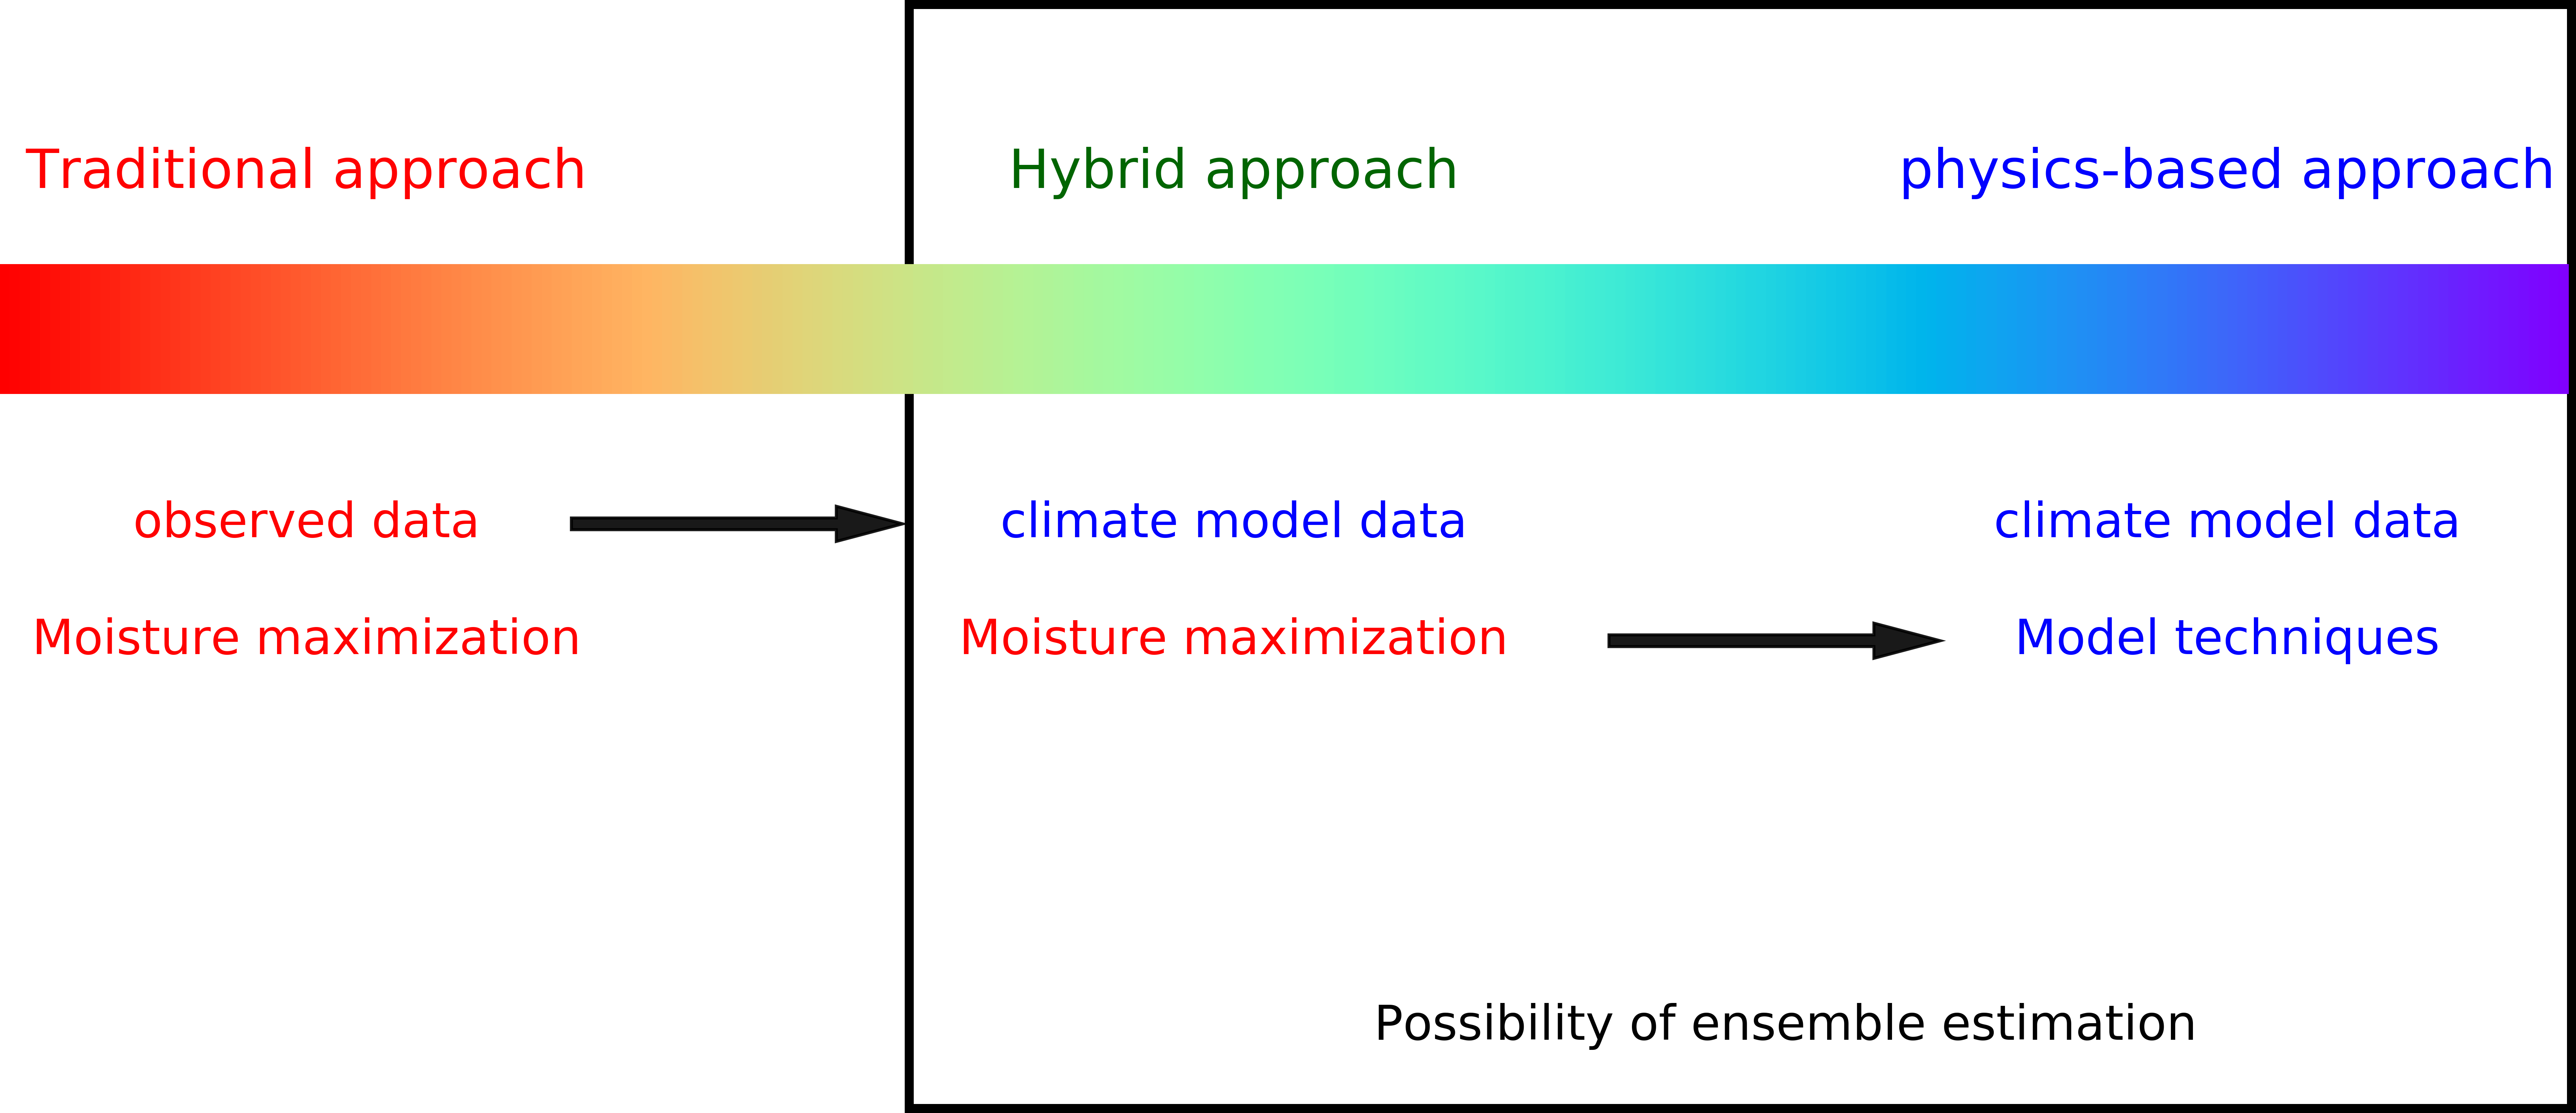
\includegraphics[width=\linewidth]{pics/ch1/fig1.png}
	\caption{A complete transition from traditional approach to physics-based approach of PMP estimation.}
    \label{fig:1-1}
\end{figure}

\section {Objectives}

Through this dissertation, I hope to have a better understanding of the relationship between extreme precipitation and the environmental conditions. Taking this information into atmospheric numerical modeling, I hope to help the engineering community to get ready to utilize atmospheric numerical models for infrastructure safety evaluation. To be specific, I hope to achieve the following goals:

1. To establish a numerical modeling framework for extreme rainfall event simulation in engineering practice.

2. To develop a method that physically estimates PMP while accounting for uncertainties for engineering practice.

3. To estimate PMP change as a function of the climate change.

\section {Approach}

The core of this dissertation is organized as follows:

Chapter \ref{ch:JHE} presents a numerical modeling framework (based on WRF) for engineering extreme precipitation events investigation. Chapter \ref{ch:EF} takes this framework and examines out capability of reconstructing the extreme precipitation events in the history. These two chapters lay the foundation of model-based storm construction and thus PMP estimation. Chapter \ref{ch:JHM} performs a statistical analysis of the extreme historical precipitation as reflected by the major reanalysis products, and reveals the spatially heterogeneous relationship between extreme precipitation and the environmental conditions. Chapter \ref{ch:WRR} develops the hybrid approach in figure \ref{fig:1-1}, and links the current and proposed PMP estimation approaches. Chapter \ref{ch:con} presents the findings from the collection of research and the recommendations of future studies.

